% !TeX program = lualatex
\documentclass[12pt]{standalone}
\usepackage{tikz}
%\usetikzlibrary{calc, arrows.meta, decorations.pathreplacing}

\begin{document}

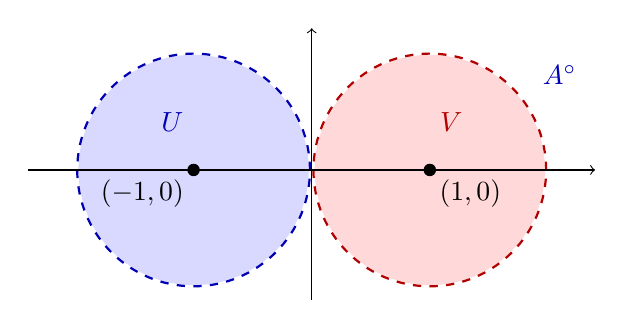
\begin{tikzpicture}[scale=1.5]
  \fill[blue!15] (-1,0) circle (0.975);
  \fill[red!15] (1,0) circle (0.975);
  \draw[blue!70!black, thick, dashed] (-1,0) circle (0.985)
    node[above left, yshift=10pt] {$U$};
  \draw[red!70!black, thick, dashed] (1,0) circle (0.985) 
    node[above right, yshift=10pt] {$V$};

  \draw[->] (-2.4,0) -- (2.4,0); % node[right] {$x$};
  \draw[->] (0,-1.1) -- (0,1.2); % node[above] {$y$};

  \fill (-1,0) circle (1.5pt) node[below left] {$(-1,0)$};
  \fill (1,0) circle (1.5pt) node[below right] {$(1,0)$};
  % \fill (0,0) circle (1.5pt) node[above right] {$0$};

  \node[blue!70!black] at (2.1, 0.8) {$A^\circ$};
\end{tikzpicture}

\end{document}
